\begin{lemma}\label{lem:simple-small-support}
Let $D\in\{3,5,7,9\}$, and let $G$ be a simple graph of maximum
degree at most $D$. If $S\subseteq E(G)$ is a clique in $L(G)^2$,
then $|S|\leq f(D)$.
\end{lemma}

\begin{proof}
Suppose that $m=f(D)+1$ marked edges form a strong clique. Any larger clique contains one of this size.
We can restrict the host to the endpoints of the marked edges, since
a joining edge for two disjoint marked edges has both endpoints in
the restriction. Write $t=\frac D2$, $r=\frac{D-1}{2}$ and
$\mu=5t^2-m=t-\frac54$. In \eqref{eq:odd-choose-anchor}, take
$\mu_*=\mu$, $g_C=\frac{99999}{100000}$ and $g_R=\frac{56425}{100000}$.
With the respective error bounds $2\cdot10^{-9}$ and $10^{-9}$ from
\eqref{eq:odd-moment-bounds}, we have $q_*>0$ for each of the four
degrees. Thus there is an induced five-cycle with all five edges marked.
Choose such a cycle minimizing $R$ in \eqref{eq:odd-core-defs}.
Denote its vertices in cyclic
order by $c_0,\ldots,c_4$ and call them the anchors. We call the
associated sets $U_0,\ldots,U_4$ the old parts. Each $U_i$ consists of the vertices whose
only neighbors on the cycle are $c_{i-1}$ and $c_{i+1}$ and whose two
edges to the cycle are marked. Set $a_i=|U_i|$, $B=\bigcup_i U_i$,
$s_i=D-a_{i-1}-a_{i+1}$, $R=\sum_i s_i$ and $A=\sum_i a_is_i$.
An \emph{old template pair} consists of two vertices, one in $U_i$
and one in $U_{i+1}$ for some $i$. The cycle vertex $c_i$ is
adjacent to every vertex in $U_{i-1}\cup U_{i+1}$, so it has
capacity for at most $s_i$ further incident edges. We call each
unit of this capacity a slot at $c_i$. We call $c_i$ saturated
when $s_i=0$. Every vertex of $U_i$ has the same bound $s_i$ on the
number of its incident edges to vertices outside $U_{i-1}\cup U_{i+1}$,
as the following adjacency property shows.
Every old template pair is an edge of $G$ by \textbf{Lemma~\ref{lem:simple-cycle-counts}}. By \eqref{eq:odd-core-sums}
and \eqref{eq:odd-core-capacity},
\[
 a_i=\frac{D-R}{2}+s_{i-2}+s_{i+2},\qquad
 e_0:=\sum_i a_i a_{i+1}=5t^2-\frac{Rt+A}{2},\qquad
 A\leq tR-\frac{1}{2}.
\]

Since $R=5D-2|B|$ is odd, \eqref{eq:odd-choose-anchor} gives
$R\leq1,5,7,7$ for $D=3,5,7,9$, respectively.
For each allowed value of $R$, the five slacks form a nonnegative
integer vector $(s_0,\ldots,s_4)$ with sum $R$. Each part contains
its anchor, so we retain a vector only if \eqref{eq:odd-core-sums}
gives $a_i\geq1$ for every $i$. Up to rotation and reflection,
the four degrees together give $1,5,16,38$ vectors for
$R=1,3,5,7$, respectively.
\textbf{Figures~\ref{fig:finite-simple-slack-low}
and~\ref{fig:finite-simple-slack-seven}} list the vectors and the degrees
that admit each one. The case $R=1$ is excluded by
\textbf{Lemma~\ref{lem:odd-unit-slack}}. For the remaining vectors we
count the marked edges on old template pairs and bound the number
of other marked edges.

\begin{figure}[htbp]
\centering
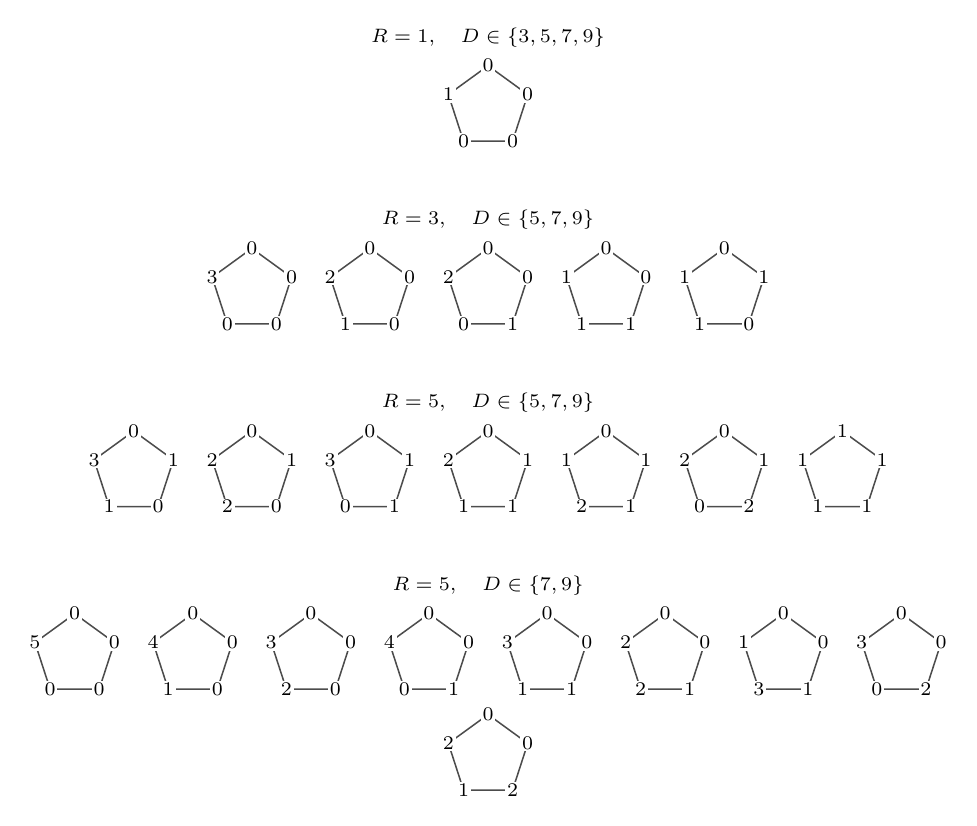
\begin{tikzpicture}[font=\scriptsize,
sc marked/.style={draw=red!65!black,line width=.75pt},
sc unmarked/.style={draw=blue!65!black,line width=.68pt,dash pattern=on 1.5pt off 1.35pt}]
\node[inner sep=0pt] at (0,0) {\(R=1,\quad D\in\{3,5,7,9\}\)};
\begin{scope}[shift={(0,-0.89)}]
\coordinate (c0) at (90:.53);
\coordinate (c1) at (18:.53);
\coordinate (c2) at (-54:.53);
\coordinate (c3) at (-126:.53);
\coordinate (c4) at (-198:.53);
\draw[black!70,line width=.55pt] (c0)--(c1)--(c2)--(c3)--(c4)--cycle;
\node[fill=white,inner sep=.65pt] at (c0) {\(0\)};
\node[fill=white,inner sep=.65pt] at (c1) {\(0\)};
\node[fill=white,inner sep=.65pt] at (c2) {\(0\)};
\node[fill=white,inner sep=.65pt] at (c3) {\(0\)};
\node[fill=white,inner sep=.65pt] at (c4) {\(1\)};
\end{scope}
\node[inner sep=0pt] at (0,-2.32) {\(R=3,\quad D\in\{5,7,9\}\)};
\begin{scope}[shift={(-3,-3.21)}]
\coordinate (c0) at (90:.53);
\coordinate (c1) at (18:.53);
\coordinate (c2) at (-54:.53);
\coordinate (c3) at (-126:.53);
\coordinate (c4) at (-198:.53);
\draw[black!70,line width=.55pt] (c0)--(c1)--(c2)--(c3)--(c4)--cycle;
\node[fill=white,inner sep=.65pt] at (c0) {\(0\)};
\node[fill=white,inner sep=.65pt] at (c1) {\(0\)};
\node[fill=white,inner sep=.65pt] at (c2) {\(0\)};
\node[fill=white,inner sep=.65pt] at (c3) {\(0\)};
\node[fill=white,inner sep=.65pt] at (c4) {\(3\)};
\end{scope}
\begin{scope}[shift={(-1.5,-3.21)}]
\coordinate (c0) at (90:.53);
\coordinate (c1) at (18:.53);
\coordinate (c2) at (-54:.53);
\coordinate (c3) at (-126:.53);
\coordinate (c4) at (-198:.53);
\draw[black!70,line width=.55pt] (c0)--(c1)--(c2)--(c3)--(c4)--cycle;
\node[fill=white,inner sep=.65pt] at (c0) {\(0\)};
\node[fill=white,inner sep=.65pt] at (c1) {\(0\)};
\node[fill=white,inner sep=.65pt] at (c2) {\(0\)};
\node[fill=white,inner sep=.65pt] at (c3) {\(1\)};
\node[fill=white,inner sep=.65pt] at (c4) {\(2\)};
\end{scope}
\begin{scope}[shift={(0,-3.21)}]
\coordinate (c0) at (90:.53);
\coordinate (c1) at (18:.53);
\coordinate (c2) at (-54:.53);
\coordinate (c3) at (-126:.53);
\coordinate (c4) at (-198:.53);
\draw[black!70,line width=.55pt] (c0)--(c1)--(c2)--(c3)--(c4)--cycle;
\node[fill=white,inner sep=.65pt] at (c0) {\(0\)};
\node[fill=white,inner sep=.65pt] at (c1) {\(0\)};
\node[fill=white,inner sep=.65pt] at (c2) {\(1\)};
\node[fill=white,inner sep=.65pt] at (c3) {\(0\)};
\node[fill=white,inner sep=.65pt] at (c4) {\(2\)};
\end{scope}
\begin{scope}[shift={(1.5,-3.21)}]
\coordinate (c0) at (90:.53);
\coordinate (c1) at (18:.53);
\coordinate (c2) at (-54:.53);
\coordinate (c3) at (-126:.53);
\coordinate (c4) at (-198:.53);
\draw[black!70,line width=.55pt] (c0)--(c1)--(c2)--(c3)--(c4)--cycle;
\node[fill=white,inner sep=.65pt] at (c0) {\(0\)};
\node[fill=white,inner sep=.65pt] at (c1) {\(0\)};
\node[fill=white,inner sep=.65pt] at (c2) {\(1\)};
\node[fill=white,inner sep=.65pt] at (c3) {\(1\)};
\node[fill=white,inner sep=.65pt] at (c4) {\(1\)};
\end{scope}
\begin{scope}[shift={(3,-3.21)}]
\coordinate (c0) at (90:.53);
\coordinate (c1) at (18:.53);
\coordinate (c2) at (-54:.53);
\coordinate (c3) at (-126:.53);
\coordinate (c4) at (-198:.53);
\draw[black!70,line width=.55pt] (c0)--(c1)--(c2)--(c3)--(c4)--cycle;
\node[fill=white,inner sep=.65pt] at (c0) {\(0\)};
\node[fill=white,inner sep=.65pt] at (c1) {\(1\)};
\node[fill=white,inner sep=.65pt] at (c2) {\(0\)};
\node[fill=white,inner sep=.65pt] at (c3) {\(1\)};
\node[fill=white,inner sep=.65pt] at (c4) {\(1\)};
\end{scope}
\node[inner sep=0pt] at (0,-4.64) {\(R=5,\quad D\in\{5,7,9\}\)};
\begin{scope}[shift={(-4.5,-5.53)}]
\coordinate (c0) at (90:.53);
\coordinate (c1) at (18:.53);
\coordinate (c2) at (-54:.53);
\coordinate (c3) at (-126:.53);
\coordinate (c4) at (-198:.53);
\draw[black!70,line width=.55pt] (c0)--(c1)--(c2)--(c3)--(c4)--cycle;
\node[fill=white,inner sep=.65pt] at (c0) {\(0\)};
\node[fill=white,inner sep=.65pt] at (c1) {\(1\)};
\node[fill=white,inner sep=.65pt] at (c2) {\(0\)};
\node[fill=white,inner sep=.65pt] at (c3) {\(1\)};
\node[fill=white,inner sep=.65pt] at (c4) {\(3\)};
\end{scope}
\begin{scope}[shift={(-3,-5.53)}]
\coordinate (c0) at (90:.53);
\coordinate (c1) at (18:.53);
\coordinate (c2) at (-54:.53);
\coordinate (c3) at (-126:.53);
\coordinate (c4) at (-198:.53);
\draw[black!70,line width=.55pt] (c0)--(c1)--(c2)--(c3)--(c4)--cycle;
\node[fill=white,inner sep=.65pt] at (c0) {\(0\)};
\node[fill=white,inner sep=.65pt] at (c1) {\(1\)};
\node[fill=white,inner sep=.65pt] at (c2) {\(0\)};
\node[fill=white,inner sep=.65pt] at (c3) {\(2\)};
\node[fill=white,inner sep=.65pt] at (c4) {\(2\)};
\end{scope}
\begin{scope}[shift={(-1.5,-5.53)}]
\coordinate (c0) at (90:.53);
\coordinate (c1) at (18:.53);
\coordinate (c2) at (-54:.53);
\coordinate (c3) at (-126:.53);
\coordinate (c4) at (-198:.53);
\draw[black!70,line width=.55pt] (c0)--(c1)--(c2)--(c3)--(c4)--cycle;
\node[fill=white,inner sep=.65pt] at (c0) {\(0\)};
\node[fill=white,inner sep=.65pt] at (c1) {\(1\)};
\node[fill=white,inner sep=.65pt] at (c2) {\(1\)};
\node[fill=white,inner sep=.65pt] at (c3) {\(0\)};
\node[fill=white,inner sep=.65pt] at (c4) {\(3\)};
\end{scope}
\begin{scope}[shift={(0,-5.53)}]
\coordinate (c0) at (90:.53);
\coordinate (c1) at (18:.53);
\coordinate (c2) at (-54:.53);
\coordinate (c3) at (-126:.53);
\coordinate (c4) at (-198:.53);
\draw[black!70,line width=.55pt] (c0)--(c1)--(c2)--(c3)--(c4)--cycle;
\node[fill=white,inner sep=.65pt] at (c0) {\(0\)};
\node[fill=white,inner sep=.65pt] at (c1) {\(1\)};
\node[fill=white,inner sep=.65pt] at (c2) {\(1\)};
\node[fill=white,inner sep=.65pt] at (c3) {\(1\)};
\node[fill=white,inner sep=.65pt] at (c4) {\(2\)};
\end{scope}
\begin{scope}[shift={(1.5,-5.53)}]
\coordinate (c0) at (90:.53);
\coordinate (c1) at (18:.53);
\coordinate (c2) at (-54:.53);
\coordinate (c3) at (-126:.53);
\coordinate (c4) at (-198:.53);
\draw[black!70,line width=.55pt] (c0)--(c1)--(c2)--(c3)--(c4)--cycle;
\node[fill=white,inner sep=.65pt] at (c0) {\(0\)};
\node[fill=white,inner sep=.65pt] at (c1) {\(1\)};
\node[fill=white,inner sep=.65pt] at (c2) {\(1\)};
\node[fill=white,inner sep=.65pt] at (c3) {\(2\)};
\node[fill=white,inner sep=.65pt] at (c4) {\(1\)};
\end{scope}
\begin{scope}[shift={(3,-5.53)}]
\coordinate (c0) at (90:.53);
\coordinate (c1) at (18:.53);
\coordinate (c2) at (-54:.53);
\coordinate (c3) at (-126:.53);
\coordinate (c4) at (-198:.53);
\draw[black!70,line width=.55pt] (c0)--(c1)--(c2)--(c3)--(c4)--cycle;
\node[fill=white,inner sep=.65pt] at (c0) {\(0\)};
\node[fill=white,inner sep=.65pt] at (c1) {\(1\)};
\node[fill=white,inner sep=.65pt] at (c2) {\(2\)};
\node[fill=white,inner sep=.65pt] at (c3) {\(0\)};
\node[fill=white,inner sep=.65pt] at (c4) {\(2\)};
\end{scope}
\begin{scope}[shift={(4.5,-5.53)}]
\coordinate (c0) at (90:.53);
\coordinate (c1) at (18:.53);
\coordinate (c2) at (-54:.53);
\coordinate (c3) at (-126:.53);
\coordinate (c4) at (-198:.53);
\draw[black!70,line width=.55pt] (c0)--(c1)--(c2)--(c3)--(c4)--cycle;
\node[fill=white,inner sep=.65pt] at (c0) {\(1\)};
\node[fill=white,inner sep=.65pt] at (c1) {\(1\)};
\node[fill=white,inner sep=.65pt] at (c2) {\(1\)};
\node[fill=white,inner sep=.65pt] at (c3) {\(1\)};
\node[fill=white,inner sep=.65pt] at (c4) {\(1\)};
\end{scope}
\node[inner sep=0pt] at (0,-6.96) {\(R=5,\quad D\in\{7,9\}\)};
\begin{scope}[shift={(-5.25,-7.85)}]
\coordinate (c0) at (90:.53);
\coordinate (c1) at (18:.53);
\coordinate (c2) at (-54:.53);
\coordinate (c3) at (-126:.53);
\coordinate (c4) at (-198:.53);
\draw[black!70,line width=.55pt] (c0)--(c1)--(c2)--(c3)--(c4)--cycle;
\node[fill=white,inner sep=.65pt] at (c0) {\(0\)};
\node[fill=white,inner sep=.65pt] at (c1) {\(0\)};
\node[fill=white,inner sep=.65pt] at (c2) {\(0\)};
\node[fill=white,inner sep=.65pt] at (c3) {\(0\)};
\node[fill=white,inner sep=.65pt] at (c4) {\(5\)};
\end{scope}
\begin{scope}[shift={(-3.75,-7.85)}]
\coordinate (c0) at (90:.53);
\coordinate (c1) at (18:.53);
\coordinate (c2) at (-54:.53);
\coordinate (c3) at (-126:.53);
\coordinate (c4) at (-198:.53);
\draw[black!70,line width=.55pt] (c0)--(c1)--(c2)--(c3)--(c4)--cycle;
\node[fill=white,inner sep=.65pt] at (c0) {\(0\)};
\node[fill=white,inner sep=.65pt] at (c1) {\(0\)};
\node[fill=white,inner sep=.65pt] at (c2) {\(0\)};
\node[fill=white,inner sep=.65pt] at (c3) {\(1\)};
\node[fill=white,inner sep=.65pt] at (c4) {\(4\)};
\end{scope}
\begin{scope}[shift={(-2.25,-7.85)}]
\coordinate (c0) at (90:.53);
\coordinate (c1) at (18:.53);
\coordinate (c2) at (-54:.53);
\coordinate (c3) at (-126:.53);
\coordinate (c4) at (-198:.53);
\draw[black!70,line width=.55pt] (c0)--(c1)--(c2)--(c3)--(c4)--cycle;
\node[fill=white,inner sep=.65pt] at (c0) {\(0\)};
\node[fill=white,inner sep=.65pt] at (c1) {\(0\)};
\node[fill=white,inner sep=.65pt] at (c2) {\(0\)};
\node[fill=white,inner sep=.65pt] at (c3) {\(2\)};
\node[fill=white,inner sep=.65pt] at (c4) {\(3\)};
\end{scope}
\begin{scope}[shift={(-0.75,-7.85)}]
\coordinate (c0) at (90:.53);
\coordinate (c1) at (18:.53);
\coordinate (c2) at (-54:.53);
\coordinate (c3) at (-126:.53);
\coordinate (c4) at (-198:.53);
\draw[black!70,line width=.55pt] (c0)--(c1)--(c2)--(c3)--(c4)--cycle;
\node[fill=white,inner sep=.65pt] at (c0) {\(0\)};
\node[fill=white,inner sep=.65pt] at (c1) {\(0\)};
\node[fill=white,inner sep=.65pt] at (c2) {\(1\)};
\node[fill=white,inner sep=.65pt] at (c3) {\(0\)};
\node[fill=white,inner sep=.65pt] at (c4) {\(4\)};
\end{scope}
\begin{scope}[shift={(0.75,-7.85)}]
\coordinate (c0) at (90:.53);
\coordinate (c1) at (18:.53);
\coordinate (c2) at (-54:.53);
\coordinate (c3) at (-126:.53);
\coordinate (c4) at (-198:.53);
\draw[black!70,line width=.55pt] (c0)--(c1)--(c2)--(c3)--(c4)--cycle;
\node[fill=white,inner sep=.65pt] at (c0) {\(0\)};
\node[fill=white,inner sep=.65pt] at (c1) {\(0\)};
\node[fill=white,inner sep=.65pt] at (c2) {\(1\)};
\node[fill=white,inner sep=.65pt] at (c3) {\(1\)};
\node[fill=white,inner sep=.65pt] at (c4) {\(3\)};
\end{scope}
\begin{scope}[shift={(2.25,-7.85)}]
\coordinate (c0) at (90:.53);
\coordinate (c1) at (18:.53);
\coordinate (c2) at (-54:.53);
\coordinate (c3) at (-126:.53);
\coordinate (c4) at (-198:.53);
\draw[black!70,line width=.55pt] (c0)--(c1)--(c2)--(c3)--(c4)--cycle;
\node[fill=white,inner sep=.65pt] at (c0) {\(0\)};
\node[fill=white,inner sep=.65pt] at (c1) {\(0\)};
\node[fill=white,inner sep=.65pt] at (c2) {\(1\)};
\node[fill=white,inner sep=.65pt] at (c3) {\(2\)};
\node[fill=white,inner sep=.65pt] at (c4) {\(2\)};
\end{scope}
\begin{scope}[shift={(3.75,-7.85)}]
\coordinate (c0) at (90:.53);
\coordinate (c1) at (18:.53);
\coordinate (c2) at (-54:.53);
\coordinate (c3) at (-126:.53);
\coordinate (c4) at (-198:.53);
\draw[black!70,line width=.55pt] (c0)--(c1)--(c2)--(c3)--(c4)--cycle;
\node[fill=white,inner sep=.65pt] at (c0) {\(0\)};
\node[fill=white,inner sep=.65pt] at (c1) {\(0\)};
\node[fill=white,inner sep=.65pt] at (c2) {\(1\)};
\node[fill=white,inner sep=.65pt] at (c3) {\(3\)};
\node[fill=white,inner sep=.65pt] at (c4) {\(1\)};
\end{scope}
\begin{scope}[shift={(5.25,-7.85)}]
\coordinate (c0) at (90:.53);
\coordinate (c1) at (18:.53);
\coordinate (c2) at (-54:.53);
\coordinate (c3) at (-126:.53);
\coordinate (c4) at (-198:.53);
\draw[black!70,line width=.55pt] (c0)--(c1)--(c2)--(c3)--(c4)--cycle;
\node[fill=white,inner sep=.65pt] at (c0) {\(0\)};
\node[fill=white,inner sep=.65pt] at (c1) {\(0\)};
\node[fill=white,inner sep=.65pt] at (c2) {\(2\)};
\node[fill=white,inner sep=.65pt] at (c3) {\(0\)};
\node[fill=white,inner sep=.65pt] at (c4) {\(3\)};
\end{scope}
\begin{scope}[shift={(0,-9.13)}]
\coordinate (c0) at (90:.53);
\coordinate (c1) at (18:.53);
\coordinate (c2) at (-54:.53);
\coordinate (c3) at (-126:.53);
\coordinate (c4) at (-198:.53);
\draw[black!70,line width=.55pt] (c0)--(c1)--(c2)--(c3)--(c4)--cycle;
\node[fill=white,inner sep=.65pt] at (c0) {\(0\)};
\node[fill=white,inner sep=.65pt] at (c1) {\(0\)};
\node[fill=white,inner sep=.65pt] at (c2) {\(2\)};
\node[fill=white,inner sep=.65pt] at (c3) {\(1\)};
\node[fill=white,inner sep=.65pt] at (c4) {\(2\)};
\end{scope}
\end{tikzpicture}
\caption{Five-cycle slack vectors with $R=1,3,5$. The five entries are read clockwise from the top. Each heading lists the degrees for which the vector satisfies the slack bound and all five parts are nonempty.}
\label{fig:finite-simple-slack-low}
\end{figure}

\begin{figure}[htbp]
\centering
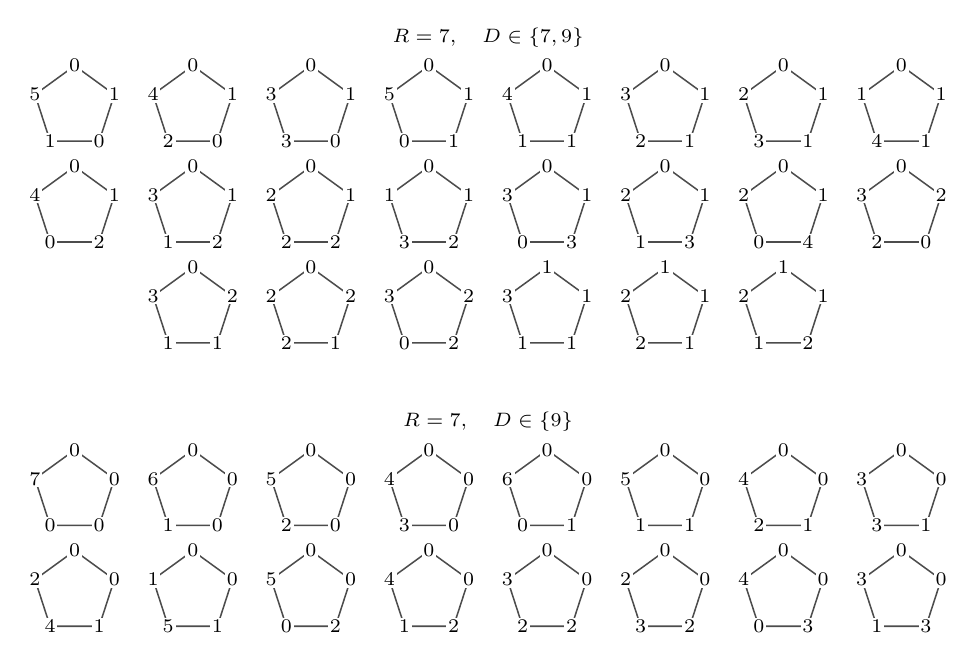
\begin{tikzpicture}[font=\scriptsize,
sc marked/.style={draw=red!65!black,line width=.75pt},
sc unmarked/.style={draw=blue!65!black,line width=.68pt,dash pattern=on 1.5pt off 1.35pt}]
\node[inner sep=0pt] at (0,0) {\(R=7,\quad D\in\{7,9\}\)};
\begin{scope}[shift={(-5.25,-0.89)}]
\coordinate (c0) at (90:.53);
\coordinate (c1) at (18:.53);
\coordinate (c2) at (-54:.53);
\coordinate (c3) at (-126:.53);
\coordinate (c4) at (-198:.53);
\draw[black!70,line width=.55pt] (c0)--(c1)--(c2)--(c3)--(c4)--cycle;
\node[fill=white,inner sep=.65pt] at (c0) {\(0\)};
\node[fill=white,inner sep=.65pt] at (c1) {\(1\)};
\node[fill=white,inner sep=.65pt] at (c2) {\(0\)};
\node[fill=white,inner sep=.65pt] at (c3) {\(1\)};
\node[fill=white,inner sep=.65pt] at (c4) {\(5\)};
\end{scope}
\begin{scope}[shift={(-3.75,-0.89)}]
\coordinate (c0) at (90:.53);
\coordinate (c1) at (18:.53);
\coordinate (c2) at (-54:.53);
\coordinate (c3) at (-126:.53);
\coordinate (c4) at (-198:.53);
\draw[black!70,line width=.55pt] (c0)--(c1)--(c2)--(c3)--(c4)--cycle;
\node[fill=white,inner sep=.65pt] at (c0) {\(0\)};
\node[fill=white,inner sep=.65pt] at (c1) {\(1\)};
\node[fill=white,inner sep=.65pt] at (c2) {\(0\)};
\node[fill=white,inner sep=.65pt] at (c3) {\(2\)};
\node[fill=white,inner sep=.65pt] at (c4) {\(4\)};
\end{scope}
\begin{scope}[shift={(-2.25,-0.89)}]
\coordinate (c0) at (90:.53);
\coordinate (c1) at (18:.53);
\coordinate (c2) at (-54:.53);
\coordinate (c3) at (-126:.53);
\coordinate (c4) at (-198:.53);
\draw[black!70,line width=.55pt] (c0)--(c1)--(c2)--(c3)--(c4)--cycle;
\node[fill=white,inner sep=.65pt] at (c0) {\(0\)};
\node[fill=white,inner sep=.65pt] at (c1) {\(1\)};
\node[fill=white,inner sep=.65pt] at (c2) {\(0\)};
\node[fill=white,inner sep=.65pt] at (c3) {\(3\)};
\node[fill=white,inner sep=.65pt] at (c4) {\(3\)};
\end{scope}
\begin{scope}[shift={(-0.75,-0.89)}]
\coordinate (c0) at (90:.53);
\coordinate (c1) at (18:.53);
\coordinate (c2) at (-54:.53);
\coordinate (c3) at (-126:.53);
\coordinate (c4) at (-198:.53);
\draw[black!70,line width=.55pt] (c0)--(c1)--(c2)--(c3)--(c4)--cycle;
\node[fill=white,inner sep=.65pt] at (c0) {\(0\)};
\node[fill=white,inner sep=.65pt] at (c1) {\(1\)};
\node[fill=white,inner sep=.65pt] at (c2) {\(1\)};
\node[fill=white,inner sep=.65pt] at (c3) {\(0\)};
\node[fill=white,inner sep=.65pt] at (c4) {\(5\)};
\end{scope}
\begin{scope}[shift={(0.75,-0.89)}]
\coordinate (c0) at (90:.53);
\coordinate (c1) at (18:.53);
\coordinate (c2) at (-54:.53);
\coordinate (c3) at (-126:.53);
\coordinate (c4) at (-198:.53);
\draw[black!70,line width=.55pt] (c0)--(c1)--(c2)--(c3)--(c4)--cycle;
\node[fill=white,inner sep=.65pt] at (c0) {\(0\)};
\node[fill=white,inner sep=.65pt] at (c1) {\(1\)};
\node[fill=white,inner sep=.65pt] at (c2) {\(1\)};
\node[fill=white,inner sep=.65pt] at (c3) {\(1\)};
\node[fill=white,inner sep=.65pt] at (c4) {\(4\)};
\end{scope}
\begin{scope}[shift={(2.25,-0.89)}]
\coordinate (c0) at (90:.53);
\coordinate (c1) at (18:.53);
\coordinate (c2) at (-54:.53);
\coordinate (c3) at (-126:.53);
\coordinate (c4) at (-198:.53);
\draw[black!70,line width=.55pt] (c0)--(c1)--(c2)--(c3)--(c4)--cycle;
\node[fill=white,inner sep=.65pt] at (c0) {\(0\)};
\node[fill=white,inner sep=.65pt] at (c1) {\(1\)};
\node[fill=white,inner sep=.65pt] at (c2) {\(1\)};
\node[fill=white,inner sep=.65pt] at (c3) {\(2\)};
\node[fill=white,inner sep=.65pt] at (c4) {\(3\)};
\end{scope}
\begin{scope}[shift={(3.75,-0.89)}]
\coordinate (c0) at (90:.53);
\coordinate (c1) at (18:.53);
\coordinate (c2) at (-54:.53);
\coordinate (c3) at (-126:.53);
\coordinate (c4) at (-198:.53);
\draw[black!70,line width=.55pt] (c0)--(c1)--(c2)--(c3)--(c4)--cycle;
\node[fill=white,inner sep=.65pt] at (c0) {\(0\)};
\node[fill=white,inner sep=.65pt] at (c1) {\(1\)};
\node[fill=white,inner sep=.65pt] at (c2) {\(1\)};
\node[fill=white,inner sep=.65pt] at (c3) {\(3\)};
\node[fill=white,inner sep=.65pt] at (c4) {\(2\)};
\end{scope}
\begin{scope}[shift={(5.25,-0.89)}]
\coordinate (c0) at (90:.53);
\coordinate (c1) at (18:.53);
\coordinate (c2) at (-54:.53);
\coordinate (c3) at (-126:.53);
\coordinate (c4) at (-198:.53);
\draw[black!70,line width=.55pt] (c0)--(c1)--(c2)--(c3)--(c4)--cycle;
\node[fill=white,inner sep=.65pt] at (c0) {\(0\)};
\node[fill=white,inner sep=.65pt] at (c1) {\(1\)};
\node[fill=white,inner sep=.65pt] at (c2) {\(1\)};
\node[fill=white,inner sep=.65pt] at (c3) {\(4\)};
\node[fill=white,inner sep=.65pt] at (c4) {\(1\)};
\end{scope}
\begin{scope}[shift={(-5.25,-2.17)}]
\coordinate (c0) at (90:.53);
\coordinate (c1) at (18:.53);
\coordinate (c2) at (-54:.53);
\coordinate (c3) at (-126:.53);
\coordinate (c4) at (-198:.53);
\draw[black!70,line width=.55pt] (c0)--(c1)--(c2)--(c3)--(c4)--cycle;
\node[fill=white,inner sep=.65pt] at (c0) {\(0\)};
\node[fill=white,inner sep=.65pt] at (c1) {\(1\)};
\node[fill=white,inner sep=.65pt] at (c2) {\(2\)};
\node[fill=white,inner sep=.65pt] at (c3) {\(0\)};
\node[fill=white,inner sep=.65pt] at (c4) {\(4\)};
\end{scope}
\begin{scope}[shift={(-3.75,-2.17)}]
\coordinate (c0) at (90:.53);
\coordinate (c1) at (18:.53);
\coordinate (c2) at (-54:.53);
\coordinate (c3) at (-126:.53);
\coordinate (c4) at (-198:.53);
\draw[black!70,line width=.55pt] (c0)--(c1)--(c2)--(c3)--(c4)--cycle;
\node[fill=white,inner sep=.65pt] at (c0) {\(0\)};
\node[fill=white,inner sep=.65pt] at (c1) {\(1\)};
\node[fill=white,inner sep=.65pt] at (c2) {\(2\)};
\node[fill=white,inner sep=.65pt] at (c3) {\(1\)};
\node[fill=white,inner sep=.65pt] at (c4) {\(3\)};
\end{scope}
\begin{scope}[shift={(-2.25,-2.17)}]
\coordinate (c0) at (90:.53);
\coordinate (c1) at (18:.53);
\coordinate (c2) at (-54:.53);
\coordinate (c3) at (-126:.53);
\coordinate (c4) at (-198:.53);
\draw[black!70,line width=.55pt] (c0)--(c1)--(c2)--(c3)--(c4)--cycle;
\node[fill=white,inner sep=.65pt] at (c0) {\(0\)};
\node[fill=white,inner sep=.65pt] at (c1) {\(1\)};
\node[fill=white,inner sep=.65pt] at (c2) {\(2\)};
\node[fill=white,inner sep=.65pt] at (c3) {\(2\)};
\node[fill=white,inner sep=.65pt] at (c4) {\(2\)};
\end{scope}
\begin{scope}[shift={(-0.75,-2.17)}]
\coordinate (c0) at (90:.53);
\coordinate (c1) at (18:.53);
\coordinate (c2) at (-54:.53);
\coordinate (c3) at (-126:.53);
\coordinate (c4) at (-198:.53);
\draw[black!70,line width=.55pt] (c0)--(c1)--(c2)--(c3)--(c4)--cycle;
\node[fill=white,inner sep=.65pt] at (c0) {\(0\)};
\node[fill=white,inner sep=.65pt] at (c1) {\(1\)};
\node[fill=white,inner sep=.65pt] at (c2) {\(2\)};
\node[fill=white,inner sep=.65pt] at (c3) {\(3\)};
\node[fill=white,inner sep=.65pt] at (c4) {\(1\)};
\end{scope}
\begin{scope}[shift={(0.75,-2.17)}]
\coordinate (c0) at (90:.53);
\coordinate (c1) at (18:.53);
\coordinate (c2) at (-54:.53);
\coordinate (c3) at (-126:.53);
\coordinate (c4) at (-198:.53);
\draw[black!70,line width=.55pt] (c0)--(c1)--(c2)--(c3)--(c4)--cycle;
\node[fill=white,inner sep=.65pt] at (c0) {\(0\)};
\node[fill=white,inner sep=.65pt] at (c1) {\(1\)};
\node[fill=white,inner sep=.65pt] at (c2) {\(3\)};
\node[fill=white,inner sep=.65pt] at (c3) {\(0\)};
\node[fill=white,inner sep=.65pt] at (c4) {\(3\)};
\end{scope}
\begin{scope}[shift={(2.25,-2.17)}]
\coordinate (c0) at (90:.53);
\coordinate (c1) at (18:.53);
\coordinate (c2) at (-54:.53);
\coordinate (c3) at (-126:.53);
\coordinate (c4) at (-198:.53);
\draw[black!70,line width=.55pt] (c0)--(c1)--(c2)--(c3)--(c4)--cycle;
\node[fill=white,inner sep=.65pt] at (c0) {\(0\)};
\node[fill=white,inner sep=.65pt] at (c1) {\(1\)};
\node[fill=white,inner sep=.65pt] at (c2) {\(3\)};
\node[fill=white,inner sep=.65pt] at (c3) {\(1\)};
\node[fill=white,inner sep=.65pt] at (c4) {\(2\)};
\end{scope}
\begin{scope}[shift={(3.75,-2.17)}]
\coordinate (c0) at (90:.53);
\coordinate (c1) at (18:.53);
\coordinate (c2) at (-54:.53);
\coordinate (c3) at (-126:.53);
\coordinate (c4) at (-198:.53);
\draw[black!70,line width=.55pt] (c0)--(c1)--(c2)--(c3)--(c4)--cycle;
\node[fill=white,inner sep=.65pt] at (c0) {\(0\)};
\node[fill=white,inner sep=.65pt] at (c1) {\(1\)};
\node[fill=white,inner sep=.65pt] at (c2) {\(4\)};
\node[fill=white,inner sep=.65pt] at (c3) {\(0\)};
\node[fill=white,inner sep=.65pt] at (c4) {\(2\)};
\end{scope}
\begin{scope}[shift={(5.25,-2.17)}]
\coordinate (c0) at (90:.53);
\coordinate (c1) at (18:.53);
\coordinate (c2) at (-54:.53);
\coordinate (c3) at (-126:.53);
\coordinate (c4) at (-198:.53);
\draw[black!70,line width=.55pt] (c0)--(c1)--(c2)--(c3)--(c4)--cycle;
\node[fill=white,inner sep=.65pt] at (c0) {\(0\)};
\node[fill=white,inner sep=.65pt] at (c1) {\(2\)};
\node[fill=white,inner sep=.65pt] at (c2) {\(0\)};
\node[fill=white,inner sep=.65pt] at (c3) {\(2\)};
\node[fill=white,inner sep=.65pt] at (c4) {\(3\)};
\end{scope}
\begin{scope}[shift={(-3.75,-3.45)}]
\coordinate (c0) at (90:.53);
\coordinate (c1) at (18:.53);
\coordinate (c2) at (-54:.53);
\coordinate (c3) at (-126:.53);
\coordinate (c4) at (-198:.53);
\draw[black!70,line width=.55pt] (c0)--(c1)--(c2)--(c3)--(c4)--cycle;
\node[fill=white,inner sep=.65pt] at (c0) {\(0\)};
\node[fill=white,inner sep=.65pt] at (c1) {\(2\)};
\node[fill=white,inner sep=.65pt] at (c2) {\(1\)};
\node[fill=white,inner sep=.65pt] at (c3) {\(1\)};
\node[fill=white,inner sep=.65pt] at (c4) {\(3\)};
\end{scope}
\begin{scope}[shift={(-2.25,-3.45)}]
\coordinate (c0) at (90:.53);
\coordinate (c1) at (18:.53);
\coordinate (c2) at (-54:.53);
\coordinate (c3) at (-126:.53);
\coordinate (c4) at (-198:.53);
\draw[black!70,line width=.55pt] (c0)--(c1)--(c2)--(c3)--(c4)--cycle;
\node[fill=white,inner sep=.65pt] at (c0) {\(0\)};
\node[fill=white,inner sep=.65pt] at (c1) {\(2\)};
\node[fill=white,inner sep=.65pt] at (c2) {\(1\)};
\node[fill=white,inner sep=.65pt] at (c3) {\(2\)};
\node[fill=white,inner sep=.65pt] at (c4) {\(2\)};
\end{scope}
\begin{scope}[shift={(-0.75,-3.45)}]
\coordinate (c0) at (90:.53);
\coordinate (c1) at (18:.53);
\coordinate (c2) at (-54:.53);
\coordinate (c3) at (-126:.53);
\coordinate (c4) at (-198:.53);
\draw[black!70,line width=.55pt] (c0)--(c1)--(c2)--(c3)--(c4)--cycle;
\node[fill=white,inner sep=.65pt] at (c0) {\(0\)};
\node[fill=white,inner sep=.65pt] at (c1) {\(2\)};
\node[fill=white,inner sep=.65pt] at (c2) {\(2\)};
\node[fill=white,inner sep=.65pt] at (c3) {\(0\)};
\node[fill=white,inner sep=.65pt] at (c4) {\(3\)};
\end{scope}
\begin{scope}[shift={(0.75,-3.45)}]
\coordinate (c0) at (90:.53);
\coordinate (c1) at (18:.53);
\coordinate (c2) at (-54:.53);
\coordinate (c3) at (-126:.53);
\coordinate (c4) at (-198:.53);
\draw[black!70,line width=.55pt] (c0)--(c1)--(c2)--(c3)--(c4)--cycle;
\node[fill=white,inner sep=.65pt] at (c0) {\(1\)};
\node[fill=white,inner sep=.65pt] at (c1) {\(1\)};
\node[fill=white,inner sep=.65pt] at (c2) {\(1\)};
\node[fill=white,inner sep=.65pt] at (c3) {\(1\)};
\node[fill=white,inner sep=.65pt] at (c4) {\(3\)};
\end{scope}
\begin{scope}[shift={(2.25,-3.45)}]
\coordinate (c0) at (90:.53);
\coordinate (c1) at (18:.53);
\coordinate (c2) at (-54:.53);
\coordinate (c3) at (-126:.53);
\coordinate (c4) at (-198:.53);
\draw[black!70,line width=.55pt] (c0)--(c1)--(c2)--(c3)--(c4)--cycle;
\node[fill=white,inner sep=.65pt] at (c0) {\(1\)};
\node[fill=white,inner sep=.65pt] at (c1) {\(1\)};
\node[fill=white,inner sep=.65pt] at (c2) {\(1\)};
\node[fill=white,inner sep=.65pt] at (c3) {\(2\)};
\node[fill=white,inner sep=.65pt] at (c4) {\(2\)};
\end{scope}
\begin{scope}[shift={(3.75,-3.45)}]
\coordinate (c0) at (90:.53);
\coordinate (c1) at (18:.53);
\coordinate (c2) at (-54:.53);
\coordinate (c3) at (-126:.53);
\coordinate (c4) at (-198:.53);
\draw[black!70,line width=.55pt] (c0)--(c1)--(c2)--(c3)--(c4)--cycle;
\node[fill=white,inner sep=.65pt] at (c0) {\(1\)};
\node[fill=white,inner sep=.65pt] at (c1) {\(1\)};
\node[fill=white,inner sep=.65pt] at (c2) {\(2\)};
\node[fill=white,inner sep=.65pt] at (c3) {\(1\)};
\node[fill=white,inner sep=.65pt] at (c4) {\(2\)};
\end{scope}
\node[inner sep=0pt] at (0,-4.88) {\(R=7,\quad D\in\{9\}\)};
\begin{scope}[shift={(-5.25,-5.77)}]
\coordinate (c0) at (90:.53);
\coordinate (c1) at (18:.53);
\coordinate (c2) at (-54:.53);
\coordinate (c3) at (-126:.53);
\coordinate (c4) at (-198:.53);
\draw[black!70,line width=.55pt] (c0)--(c1)--(c2)--(c3)--(c4)--cycle;
\node[fill=white,inner sep=.65pt] at (c0) {\(0\)};
\node[fill=white,inner sep=.65pt] at (c1) {\(0\)};
\node[fill=white,inner sep=.65pt] at (c2) {\(0\)};
\node[fill=white,inner sep=.65pt] at (c3) {\(0\)};
\node[fill=white,inner sep=.65pt] at (c4) {\(7\)};
\end{scope}
\begin{scope}[shift={(-3.75,-5.77)}]
\coordinate (c0) at (90:.53);
\coordinate (c1) at (18:.53);
\coordinate (c2) at (-54:.53);
\coordinate (c3) at (-126:.53);
\coordinate (c4) at (-198:.53);
\draw[black!70,line width=.55pt] (c0)--(c1)--(c2)--(c3)--(c4)--cycle;
\node[fill=white,inner sep=.65pt] at (c0) {\(0\)};
\node[fill=white,inner sep=.65pt] at (c1) {\(0\)};
\node[fill=white,inner sep=.65pt] at (c2) {\(0\)};
\node[fill=white,inner sep=.65pt] at (c3) {\(1\)};
\node[fill=white,inner sep=.65pt] at (c4) {\(6\)};
\end{scope}
\begin{scope}[shift={(-2.25,-5.77)}]
\coordinate (c0) at (90:.53);
\coordinate (c1) at (18:.53);
\coordinate (c2) at (-54:.53);
\coordinate (c3) at (-126:.53);
\coordinate (c4) at (-198:.53);
\draw[black!70,line width=.55pt] (c0)--(c1)--(c2)--(c3)--(c4)--cycle;
\node[fill=white,inner sep=.65pt] at (c0) {\(0\)};
\node[fill=white,inner sep=.65pt] at (c1) {\(0\)};
\node[fill=white,inner sep=.65pt] at (c2) {\(0\)};
\node[fill=white,inner sep=.65pt] at (c3) {\(2\)};
\node[fill=white,inner sep=.65pt] at (c4) {\(5\)};
\end{scope}
\begin{scope}[shift={(-0.75,-5.77)}]
\coordinate (c0) at (90:.53);
\coordinate (c1) at (18:.53);
\coordinate (c2) at (-54:.53);
\coordinate (c3) at (-126:.53);
\coordinate (c4) at (-198:.53);
\draw[black!70,line width=.55pt] (c0)--(c1)--(c2)--(c3)--(c4)--cycle;
\node[fill=white,inner sep=.65pt] at (c0) {\(0\)};
\node[fill=white,inner sep=.65pt] at (c1) {\(0\)};
\node[fill=white,inner sep=.65pt] at (c2) {\(0\)};
\node[fill=white,inner sep=.65pt] at (c3) {\(3\)};
\node[fill=white,inner sep=.65pt] at (c4) {\(4\)};
\end{scope}
\begin{scope}[shift={(0.75,-5.77)}]
\coordinate (c0) at (90:.53);
\coordinate (c1) at (18:.53);
\coordinate (c2) at (-54:.53);
\coordinate (c3) at (-126:.53);
\coordinate (c4) at (-198:.53);
\draw[black!70,line width=.55pt] (c0)--(c1)--(c2)--(c3)--(c4)--cycle;
\node[fill=white,inner sep=.65pt] at (c0) {\(0\)};
\node[fill=white,inner sep=.65pt] at (c1) {\(0\)};
\node[fill=white,inner sep=.65pt] at (c2) {\(1\)};
\node[fill=white,inner sep=.65pt] at (c3) {\(0\)};
\node[fill=white,inner sep=.65pt] at (c4) {\(6\)};
\end{scope}
\begin{scope}[shift={(2.25,-5.77)}]
\coordinate (c0) at (90:.53);
\coordinate (c1) at (18:.53);
\coordinate (c2) at (-54:.53);
\coordinate (c3) at (-126:.53);
\coordinate (c4) at (-198:.53);
\draw[black!70,line width=.55pt] (c0)--(c1)--(c2)--(c3)--(c4)--cycle;
\node[fill=white,inner sep=.65pt] at (c0) {\(0\)};
\node[fill=white,inner sep=.65pt] at (c1) {\(0\)};
\node[fill=white,inner sep=.65pt] at (c2) {\(1\)};
\node[fill=white,inner sep=.65pt] at (c3) {\(1\)};
\node[fill=white,inner sep=.65pt] at (c4) {\(5\)};
\end{scope}
\begin{scope}[shift={(3.75,-5.77)}]
\coordinate (c0) at (90:.53);
\coordinate (c1) at (18:.53);
\coordinate (c2) at (-54:.53);
\coordinate (c3) at (-126:.53);
\coordinate (c4) at (-198:.53);
\draw[black!70,line width=.55pt] (c0)--(c1)--(c2)--(c3)--(c4)--cycle;
\node[fill=white,inner sep=.65pt] at (c0) {\(0\)};
\node[fill=white,inner sep=.65pt] at (c1) {\(0\)};
\node[fill=white,inner sep=.65pt] at (c2) {\(1\)};
\node[fill=white,inner sep=.65pt] at (c3) {\(2\)};
\node[fill=white,inner sep=.65pt] at (c4) {\(4\)};
\end{scope}
\begin{scope}[shift={(5.25,-5.77)}]
\coordinate (c0) at (90:.53);
\coordinate (c1) at (18:.53);
\coordinate (c2) at (-54:.53);
\coordinate (c3) at (-126:.53);
\coordinate (c4) at (-198:.53);
\draw[black!70,line width=.55pt] (c0)--(c1)--(c2)--(c3)--(c4)--cycle;
\node[fill=white,inner sep=.65pt] at (c0) {\(0\)};
\node[fill=white,inner sep=.65pt] at (c1) {\(0\)};
\node[fill=white,inner sep=.65pt] at (c2) {\(1\)};
\node[fill=white,inner sep=.65pt] at (c3) {\(3\)};
\node[fill=white,inner sep=.65pt] at (c4) {\(3\)};
\end{scope}
\begin{scope}[shift={(-5.25,-7.05)}]
\coordinate (c0) at (90:.53);
\coordinate (c1) at (18:.53);
\coordinate (c2) at (-54:.53);
\coordinate (c3) at (-126:.53);
\coordinate (c4) at (-198:.53);
\draw[black!70,line width=.55pt] (c0)--(c1)--(c2)--(c3)--(c4)--cycle;
\node[fill=white,inner sep=.65pt] at (c0) {\(0\)};
\node[fill=white,inner sep=.65pt] at (c1) {\(0\)};
\node[fill=white,inner sep=.65pt] at (c2) {\(1\)};
\node[fill=white,inner sep=.65pt] at (c3) {\(4\)};
\node[fill=white,inner sep=.65pt] at (c4) {\(2\)};
\end{scope}
\begin{scope}[shift={(-3.75,-7.05)}]
\coordinate (c0) at (90:.53);
\coordinate (c1) at (18:.53);
\coordinate (c2) at (-54:.53);
\coordinate (c3) at (-126:.53);
\coordinate (c4) at (-198:.53);
\draw[black!70,line width=.55pt] (c0)--(c1)--(c2)--(c3)--(c4)--cycle;
\node[fill=white,inner sep=.65pt] at (c0) {\(0\)};
\node[fill=white,inner sep=.65pt] at (c1) {\(0\)};
\node[fill=white,inner sep=.65pt] at (c2) {\(1\)};
\node[fill=white,inner sep=.65pt] at (c3) {\(5\)};
\node[fill=white,inner sep=.65pt] at (c4) {\(1\)};
\end{scope}
\begin{scope}[shift={(-2.25,-7.05)}]
\coordinate (c0) at (90:.53);
\coordinate (c1) at (18:.53);
\coordinate (c2) at (-54:.53);
\coordinate (c3) at (-126:.53);
\coordinate (c4) at (-198:.53);
\draw[black!70,line width=.55pt] (c0)--(c1)--(c2)--(c3)--(c4)--cycle;
\node[fill=white,inner sep=.65pt] at (c0) {\(0\)};
\node[fill=white,inner sep=.65pt] at (c1) {\(0\)};
\node[fill=white,inner sep=.65pt] at (c2) {\(2\)};
\node[fill=white,inner sep=.65pt] at (c3) {\(0\)};
\node[fill=white,inner sep=.65pt] at (c4) {\(5\)};
\end{scope}
\begin{scope}[shift={(-0.75,-7.05)}]
\coordinate (c0) at (90:.53);
\coordinate (c1) at (18:.53);
\coordinate (c2) at (-54:.53);
\coordinate (c3) at (-126:.53);
\coordinate (c4) at (-198:.53);
\draw[black!70,line width=.55pt] (c0)--(c1)--(c2)--(c3)--(c4)--cycle;
\node[fill=white,inner sep=.65pt] at (c0) {\(0\)};
\node[fill=white,inner sep=.65pt] at (c1) {\(0\)};
\node[fill=white,inner sep=.65pt] at (c2) {\(2\)};
\node[fill=white,inner sep=.65pt] at (c3) {\(1\)};
\node[fill=white,inner sep=.65pt] at (c4) {\(4\)};
\end{scope}
\begin{scope}[shift={(0.75,-7.05)}]
\coordinate (c0) at (90:.53);
\coordinate (c1) at (18:.53);
\coordinate (c2) at (-54:.53);
\coordinate (c3) at (-126:.53);
\coordinate (c4) at (-198:.53);
\draw[black!70,line width=.55pt] (c0)--(c1)--(c2)--(c3)--(c4)--cycle;
\node[fill=white,inner sep=.65pt] at (c0) {\(0\)};
\node[fill=white,inner sep=.65pt] at (c1) {\(0\)};
\node[fill=white,inner sep=.65pt] at (c2) {\(2\)};
\node[fill=white,inner sep=.65pt] at (c3) {\(2\)};
\node[fill=white,inner sep=.65pt] at (c4) {\(3\)};
\end{scope}
\begin{scope}[shift={(2.25,-7.05)}]
\coordinate (c0) at (90:.53);
\coordinate (c1) at (18:.53);
\coordinate (c2) at (-54:.53);
\coordinate (c3) at (-126:.53);
\coordinate (c4) at (-198:.53);
\draw[black!70,line width=.55pt] (c0)--(c1)--(c2)--(c3)--(c4)--cycle;
\node[fill=white,inner sep=.65pt] at (c0) {\(0\)};
\node[fill=white,inner sep=.65pt] at (c1) {\(0\)};
\node[fill=white,inner sep=.65pt] at (c2) {\(2\)};
\node[fill=white,inner sep=.65pt] at (c3) {\(3\)};
\node[fill=white,inner sep=.65pt] at (c4) {\(2\)};
\end{scope}
\begin{scope}[shift={(3.75,-7.05)}]
\coordinate (c0) at (90:.53);
\coordinate (c1) at (18:.53);
\coordinate (c2) at (-54:.53);
\coordinate (c3) at (-126:.53);
\coordinate (c4) at (-198:.53);
\draw[black!70,line width=.55pt] (c0)--(c1)--(c2)--(c3)--(c4)--cycle;
\node[fill=white,inner sep=.65pt] at (c0) {\(0\)};
\node[fill=white,inner sep=.65pt] at (c1) {\(0\)};
\node[fill=white,inner sep=.65pt] at (c2) {\(3\)};
\node[fill=white,inner sep=.65pt] at (c3) {\(0\)};
\node[fill=white,inner sep=.65pt] at (c4) {\(4\)};
\end{scope}
\begin{scope}[shift={(5.25,-7.05)}]
\coordinate (c0) at (90:.53);
\coordinate (c1) at (18:.53);
\coordinate (c2) at (-54:.53);
\coordinate (c3) at (-126:.53);
\coordinate (c4) at (-198:.53);
\draw[black!70,line width=.55pt] (c0)--(c1)--(c2)--(c3)--(c4)--cycle;
\node[fill=white,inner sep=.65pt] at (c0) {\(0\)};
\node[fill=white,inner sep=.65pt] at (c1) {\(0\)};
\node[fill=white,inner sep=.65pt] at (c2) {\(3\)};
\node[fill=white,inner sep=.65pt] at (c3) {\(1\)};
\node[fill=white,inner sep=.65pt] at (c4) {\(3\)};
\end{scope}
\end{tikzpicture}
\caption{Five-cycle slack vectors with $R=7$. The five entries are read clockwise from the top. Each heading lists the degrees for which the vector satisfies the slack bound and all five parts are nonempty.}
\label{fig:finite-simple-slack-seven}
\end{figure}


Let $\nu$ count the unmarked old template edges and let $J$ count the
marked edges with both endpoints outside $B$. For $x\notin B$, write
$S(x)=\{i:xc_i\in E(G)\}$ for its set of neighbors on the cycle,
represented by their indices. We call $S(x)$ the signature of $x$.
For a single vertex there are eight possibilities up to rotation and
reflection, as shown in \textbf{Figure~\ref{fig:finite-simple-signatures}}.
Once $(s_0,\ldots,s_4)$ is fixed, a neighbor at $c_i$ uses one of the
$s_i$ available incidences there. We therefore keep the actual index of
each neighbor and use the same cyclic ordering for all exterior vertices.

\begin{figure}[htbp]
\centering
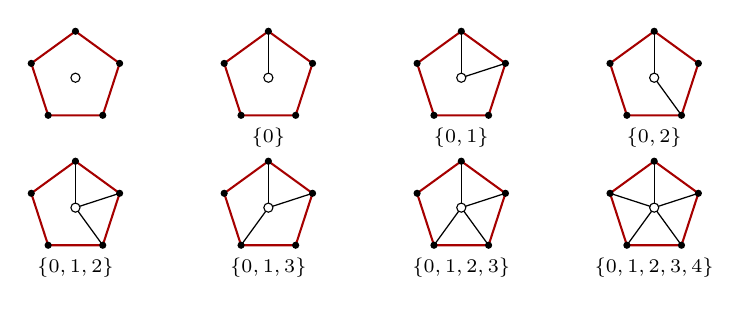
\begin{tikzpicture}[font=\scriptsize,
sc marked/.style={draw=red!65!black,line width=.75pt},
sc unmarked/.style={draw=blue!65!black,line width=.68pt,dash pattern=on 1.5pt off 1.35pt}]
\begin{scope}[shift={(-3.675,0)}]
\coordinate (c0) at (90:.59);
\coordinate (c1) at (18:.59);
\coordinate (c2) at (-54:.59);
\coordinate (c3) at (-126:.59);
\coordinate (c4) at (-198:.59);
\draw[sc marked] (c0)--(c1)--(c2)--(c3)--(c4)--cycle;
\fill (c0) circle[radius=1.3pt];
\fill (c1) circle[radius=1.3pt];
\fill (c2) circle[radius=1.3pt];
\fill (c3) circle[radius=1.3pt];
\fill (c4) circle[radius=1.3pt];
\draw[fill=white] (0,0) circle[radius=1.65pt];
\node at (0,-.76) {\(\varnothing\)};
\end{scope}
\begin{scope}[shift={(-1.225,0)}]
\coordinate (c0) at (90:.59);
\coordinate (c1) at (18:.59);
\coordinate (c2) at (-54:.59);
\coordinate (c3) at (-126:.59);
\coordinate (c4) at (-198:.59);
\draw[sc marked] (c0)--(c1)--(c2)--(c3)--(c4)--cycle;
\draw[black,line width=.45pt] (0,0)--(c0);
\fill (c0) circle[radius=1.3pt];
\fill (c1) circle[radius=1.3pt];
\fill (c2) circle[radius=1.3pt];
\fill (c3) circle[radius=1.3pt];
\fill (c4) circle[radius=1.3pt];
\draw[fill=white] (0,0) circle[radius=1.65pt];
\node at (0,-.76) {\(\{0\}\)};
\end{scope}
\begin{scope}[shift={(1.225,0)}]
\coordinate (c0) at (90:.59);
\coordinate (c1) at (18:.59);
\coordinate (c2) at (-54:.59);
\coordinate (c3) at (-126:.59);
\coordinate (c4) at (-198:.59);
\draw[sc marked] (c0)--(c1)--(c2)--(c3)--(c4)--cycle;
\draw[black,line width=.45pt] (0,0)--(c0);
\draw[black,line width=.45pt] (0,0)--(c1);
\fill (c0) circle[radius=1.3pt];
\fill (c1) circle[radius=1.3pt];
\fill (c2) circle[radius=1.3pt];
\fill (c3) circle[radius=1.3pt];
\fill (c4) circle[radius=1.3pt];
\draw[fill=white] (0,0) circle[radius=1.65pt];
\node at (0,-.76) {\(\{0,1\}\)};
\end{scope}
\begin{scope}[shift={(3.675,0)}]
\coordinate (c0) at (90:.59);
\coordinate (c1) at (18:.59);
\coordinate (c2) at (-54:.59);
\coordinate (c3) at (-126:.59);
\coordinate (c4) at (-198:.59);
\draw[sc marked] (c0)--(c1)--(c2)--(c3)--(c4)--cycle;
\draw[black,line width=.45pt] (0,0)--(c0);
\draw[black,line width=.45pt] (0,0)--(c2);
\fill (c0) circle[radius=1.3pt];
\fill (c1) circle[radius=1.3pt];
\fill (c2) circle[radius=1.3pt];
\fill (c3) circle[radius=1.3pt];
\fill (c4) circle[radius=1.3pt];
\draw[fill=white] (0,0) circle[radius=1.65pt];
\node at (0,-.76) {\(\{0,2\}\)};
\end{scope}
\begin{scope}[shift={(-3.675,-1.65)}]
\coordinate (c0) at (90:.59);
\coordinate (c1) at (18:.59);
\coordinate (c2) at (-54:.59);
\coordinate (c3) at (-126:.59);
\coordinate (c4) at (-198:.59);
\draw[sc marked] (c0)--(c1)--(c2)--(c3)--(c4)--cycle;
\draw[black,line width=.45pt] (0,0)--(c0);
\draw[black,line width=.45pt] (0,0)--(c1);
\draw[black,line width=.45pt] (0,0)--(c2);
\fill (c0) circle[radius=1.3pt];
\fill (c1) circle[radius=1.3pt];
\fill (c2) circle[radius=1.3pt];
\fill (c3) circle[radius=1.3pt];
\fill (c4) circle[radius=1.3pt];
\draw[fill=white] (0,0) circle[radius=1.65pt];
\node at (0,-.76) {\(\{0,1,2\}\)};
\end{scope}
\begin{scope}[shift={(-1.225,-1.65)}]
\coordinate (c0) at (90:.59);
\coordinate (c1) at (18:.59);
\coordinate (c2) at (-54:.59);
\coordinate (c3) at (-126:.59);
\coordinate (c4) at (-198:.59);
\draw[sc marked] (c0)--(c1)--(c2)--(c3)--(c4)--cycle;
\draw[black,line width=.45pt] (0,0)--(c0);
\draw[black,line width=.45pt] (0,0)--(c1);
\draw[black,line width=.45pt] (0,0)--(c3);
\fill (c0) circle[radius=1.3pt];
\fill (c1) circle[radius=1.3pt];
\fill (c2) circle[radius=1.3pt];
\fill (c3) circle[radius=1.3pt];
\fill (c4) circle[radius=1.3pt];
\draw[fill=white] (0,0) circle[radius=1.65pt];
\node at (0,-.76) {\(\{0,1,3\}\)};
\end{scope}
\begin{scope}[shift={(1.225,-1.65)}]
\coordinate (c0) at (90:.59);
\coordinate (c1) at (18:.59);
\coordinate (c2) at (-54:.59);
\coordinate (c3) at (-126:.59);
\coordinate (c4) at (-198:.59);
\draw[sc marked] (c0)--(c1)--(c2)--(c3)--(c4)--cycle;
\draw[black,line width=.45pt] (0,0)--(c0);
\draw[black,line width=.45pt] (0,0)--(c1);
\draw[black,line width=.45pt] (0,0)--(c2);
\draw[black,line width=.45pt] (0,0)--(c3);
\fill (c0) circle[radius=1.3pt];
\fill (c1) circle[radius=1.3pt];
\fill (c2) circle[radius=1.3pt];
\fill (c3) circle[radius=1.3pt];
\fill (c4) circle[radius=1.3pt];
\draw[fill=white] (0,0) circle[radius=1.65pt];
\node at (0,-.76) {\(\{0,1,2,3\}\)};
\end{scope}
\begin{scope}[shift={(3.675,-1.65)}]
\coordinate (c0) at (90:.59);
\coordinate (c1) at (18:.59);
\coordinate (c2) at (-54:.59);
\coordinate (c3) at (-126:.59);
\coordinate (c4) at (-198:.59);
\draw[sc marked] (c0)--(c1)--(c2)--(c3)--(c4)--cycle;
\draw[black,line width=.45pt] (0,0)--(c0);
\draw[black,line width=.45pt] (0,0)--(c1);
\draw[black,line width=.45pt] (0,0)--(c2);
\draw[black,line width=.45pt] (0,0)--(c3);
\draw[black,line width=.45pt] (0,0)--(c4);
\fill (c0) circle[radius=1.3pt];
\fill (c1) circle[radius=1.3pt];
\fill (c2) circle[radius=1.3pt];
\fill (c3) circle[radius=1.3pt];
\fill (c4) circle[radius=1.3pt];
\draw[fill=white] (0,0) circle[radius=1.65pt];
\node at (0,-.76) {\(\{0,1,2,3,4\}\)};
\end{scope}
\end{tikzpicture}
\caption{The eight possible neighborhoods of one exterior vertex on the cycle, up to rotation and reflection. The open vertex is $x$. The cycle vertices are indexed clockwise from the top. A spoke indicates adjacency to $x$ and can be marked or unmarked.}
\label{fig:finite-simple-signatures}
\end{figure}


If $xy$ is a marked edge outside $B$, then $S(x)\cup S(y)$ covers
the edges of the cycle. A vertex cover of a five-cycle has at least
three vertices, so
\begin{equation}\label{eq:odd-interior-slots}
 \sum_{x\notin B}|S(x)|\leq R,\qquad 3J\leq R(D-1).
\end{equation}
The second bound follows by summing $|S(x)|+|S(y)|$ over the $J$
edges and using that $x$ has at most $D-|S(x)|$ neighbors outside $B$.
If at most $n_0$ vertices are incident with these edges, each such
vertex has degree at most $n_0-1$ in their graph, giving
$3J\leq(n_0-1)R$ when $n_0\geq1$. There are at most $A$ marked
edges meeting $B$ outside the old template pairs, since each uses
at least one of the $A$ available incidences in $B$. Thus
$m\leq e_0-\nu+A+J$, from which
$\nu\leq \mu_*+J-\frac{Rt-A}{2}\leq r-1+J$.

Suppose $a_*=\frac{D-R}{2}>0$. If an independent set in the marked
graph on $B$ contains $x_i$ vertices of $U_i$, every pair between
consecutive parts in this set is unmarked, so $\sum_i x_ix_{i+1}\leq \nu$.
We have $\sum_i x_ix_{i+1}\geq a_*(\sum_i x_i-D)$ for
$0\leq x_i\leq a_i$. The difference of the two sides is affine in each
coordinate with the others fixed, so it attains its minimum at a corner.
At a corner, if both parts of a consecutive pair are occupied, remove
one of the two parts. Charge each removal to its consecutive pair.
Since every $a_i\geq a_*$, a removal of $U_i$ charged to $U_i,U_{i+1}$
costs $a_i\leq\frac{a_ia_{i+1}}{a_*}$, and the same inequality holds
with the indices reversed. The surviving parts are nonconsecutive
and have total size at most $D$, by \eqref{eq:odd-core-defs}.
The claim bounds the size of the independent set by $D+\frac{\nu}{a_*}$.
Thus, if $\nu\leq \nu_+$, every vertex cover of the marked graph on $B$
has size at least
\[
 C=\left\lceil \frac{3D-R}{2}-\frac{\nu_+}{a_*}\right\rceil.
\]
The neighborhoods in $B$ of the endpoints of any marked edge
outside $B$ form a vertex cover of the marked graph on $B$.
When $C>D$, each such endpoint therefore has at least $C-D$
neighbors in $B$. There are at most
$n_0=\bigl\lfloor\frac{A}{C-D}\bigr\rfloor$ such endpoints. Summing their
neighborhood sizes over the $J$ edges gives $CJ\leq\max(0,n_0-1)A$.
Starting with
$\nu_+=r-1+\lfloor \frac{R(D-1)}{3}\rfloor$, we iteratively lower $\nu_+$ using
$\nu\leq r-1+J$ and
\[
 J\leq \min\left\{\binom{n_0}{2},
       \left\lfloor\frac{\max(0,n_0-1)A}{C}\right\rfloor,
       \left\lfloor\frac{\max(0,n_0-1)R}{3}\right\rfloor\right\}.
\]
For $n_0=0$ the bound on $J$ is zero. The inequality $A\leq\frac{DR-1}{2}$ also permits us to use
$\lfloor\frac{DR-1}{2}\rfloor$ in place of $A$.

Fix an interval $\nu_-\leq \nu\leq \nu_+$, let
$L=a_*-\lfloor\sqrt{\nu_+}\rfloor$ and put $\beta=D-2L$.
For $x\notin B$, call an old part \emph{nearly full for $x$} if
$x$ has at least $L$ neighbors there. A marked edge $xy$ with $y\in U_i$
requires
$S(x)\cap\{i+2,i+3\}\ne\varnothing$. If the intersection is
$\{j\}$, let $k$ be the other index in $\{i+2,i+3\}$. Compare
$xy$ with the marked edges from $c_k$ to every vertex of $U_j$. This gives at least $a_j-s_i\geq a_*$ neighbors
of $x$ in $U_j$. In all cases, at least one of $U_{i+2}$ and $U_{i+3}$
is nearly full for $x$. Otherwise each $U_j$ with
$j\in\{i+2,i+3\}$ contains at least $a_j-L+1$ nonneighbors of $x$.
After removing the neighbors of $y$, at least $a_j-L+1-s_i\geq
a_*-L+1$ vertices remain in each part. As
$(a_*-L+1)^2>\nu_+$, a marked edge joins the two remaining sets.
This contradicts that the edge and $xy$ belong to the same strong clique.

A vertex qualifies for part $i$ if its marked degrees into
$U_{i-1}$ and $U_{i+1}$ exceed $s_{i+1}+s_{i+2}$ and
$s_{i-1}+s_{i-2}$, respectively. Add each exterior vertex satisfying
either of the following conditions to an eligible part $i$.
\begin{enumerate}[label=(\roman*)]
\item Its signature is exactly $\{i-1,i+1\}$ and it qualifies for $i$.
      The marked-star comparison above gives at least $a_*$ host
      neighbors in each specified part.
\item Its signature has size at least $3$ and contains $\{i-1,i+1\}$,
      both specified parts are nearly full for this vertex,
      and it qualifies for $i$.
\end{enumerate}
Assign each eligible vertex to one part. Let $k$ be the number of
added vertices. Let $k_1$ and $k_2$ count those with one and with at least
two neighbors on the cycle in addition to the two specified anchors.
Write $U'_i$ for the enlarged parts, $B'=\bigcup_i U'_i$,
$a'_i=|U'_i|$, $s'_i=D-a'_{i-1}-a'_{i+1}$, $A'=\sum_i a'_is'_i$,
and $e'_0=\sum_i a'_ia'_{i+1}$. Every added vertex is adjacent to its two
specified anchors, so $s'_i\geq0$ and $R':=\sum_i s'_i=R-2k$.
At $c_i$, the corresponding number of slots after enlargement is $s'_i$.
The signature sizes of the vertices outside $B'$ sum to at most
$R'-k_1-2k_2$.

An \emph{enlarged template pair} consists of a vertex of $U'_i$
and a vertex of $U'_{i+1}$ for some $i$. Let $E_0$ and $E_1$
count the enlarged template pairs absent
from $G$ that have one and two new endpoints, respectively, and set
$E=E_0+E_1$. Let $V$ count the unmarked enlarged template edges with
at least one new endpoint. If $x$ was added to $U'_i$ and is nonadjacent to
$y\in U_{i+1}$, select a marked $xu$ with $u\in U_{i-1}$ and
$u\not\sim_G y$, using qualification. Comparison with $yc_{i+2}$
forces $i+2\in S(x)$. Write $N_G(v)$ for the set of neighbors of
$v$ in $G$. Comparing $xu$ with all marked edges from $y$ into
$U_{i+2}$ puts their other endpoints in $N_G(x)\cup N_G(u)$.
It follows that the missing pair has at least $a_*-\beta$ unmarked edges
to charge at $y$ in this direction. When $x$ has just one extra anchor
incidence, it is adjacent to every vertex of $U_{i-1}$. In this case the charge
is at least $L-R$. Alternatively, $u$ has at most
$s'_{i-1}+k_1+k_2-1$ host neighbors outside the template pairs
incident with it. This gives a charge of at least
$L-k+3-R'-k_1-k_2$, since the incidence $xc_{i+2}$ uses an enlarged
slot outside parts $i+3,i-1$, and $s_{i+3}\leq s'_{i+3}+k-1$.
The opposite direction follows by reversing the indices. Hence set
\[
 \ell_1=\max\{L-R,L-k+3-R'-k_1-k_2\},\qquad \ell_2=a_*-\beta.
\]
For fixed $x$, each old unmarked edge pays at most once, as its endpoint
in the intended part determines the missing pair and direction.
Regardless of the charge, each of the $k_1$ vertices lacks at most
$\frac{D+R}{2}-L$ old template edges and each of the $k_2$ vertices at
most $\beta$. With positive charges one can thus take the lesser of this
absolute bound and $\lfloor(\frac{k_1}{\ell_1}+\frac{k_2}{\ell_2})\nu_+\rfloor$ for
$E_{0,*}\geq E_0$. A summand with zero numerator is omitted. If
$\ell_2\leq0$ and $k_2>0$, use the absolute bound for those vertices and
the lesser of the two bounds for the others. The corresponding lower
bound $B_*$ for $\nu-E_0$ is $\nu_--E_{0,*}$. When both classes of added
vertices with nonzero counts have positive charges, we may replace
$B_*$ by the larger of this bound and
$\min_{\nu_-\leq \nu\leq \nu_+}\bigl\lceil
(1-\frac{k_1}{\ell_1}-\frac{k_2}{\ell_2})\nu\bigr\rceil$,
with zero-numerator terms omitted.

Suppose $x\in U'_i\setminus U_i$ and $y\in U'_{i+1}\setminus U_{i+1}$
are adjacent to every vertex of their two specified old parts.
Then $y$ has at most $s_{i+1}$ neighbors outside its specified parts,
so the qualification condition lets us choose a marked edge $xu$
with $u\in U_{i-1}$ nonadjacent to $y$. Also $x$ has at most $s_i$
neighbors outside its specified parts and $u$ has at most $s_{i-1}$
neighbors outside its two consecutive old parts. Thus we may choose a
marked edge $yv$ with $v\in U_{i+2}$ adjacent to neither $x$ nor $u$.
If $x$ and $y$ were nonadjacent, $xu$ and $yv$ could not belong to
the same strong clique. Consequently
\[
 E_1\leq E_{1,*}:=\min\{\lfloor \frac{k^2}{4}\rfloor,\,
 k_1' (k-k_1')+\binom{k_1'}{2},\,(k-1)E_{0,*}\},
 \qquad k_1'=k_1+k_2 ,
\]
with $E_{1,*}=0$ for $k=0$. The first bound is the edge bound for the
five-cycle weighted by the numbers of new vertices in the parts.
The second counts the pairs with at least one endpoint with an extra
anchor incidence. The third counts pairs having an endpoint incident
with a missing old--new pair. If $2(L-\beta)\geq R$, we can charge
each missing new--new pair to the unmarked edges counted by $V$.
Indeed, comparing edges in
the two orders gives either one opposite marked degree at most $\beta$ or
the sum of the two opposite unmarked degrees at least
$2(L-\beta)-s_{i-1}-s_{i+2}\geq k_i+k_{i+1}$ for an $i,i+1$ pair,
where $k_i=|U'_i\setminus U_i|$. In the first case the single unmarked
degree is at least $L-\beta\geq \frac{R}{2}>k$. Dividing the relevant unmarked
degrees among their potential partners pays each possible missing
pair at least one unit. Let $E_{1,\mathrm{fee}}=0$ when these charges
are available and $E_{1,*}$ otherwise. In particular,
$\nu+V-E\geq B_*-E_{1,\mathrm{fee}}$.

If $R'=1$, there is a unique index $i$ with $s'_i=1$. The anchors
in the other four parts have degree $D$ to their consecutive enlarged
parts. No endpoint in $U'_i$ or outside $B'$ can meet or be adjacent
to an endpoint of $c_{i+2}c_{i+3}$. Thus each marked edge outside the
enlarged template pairs meets a part with $s'_j=0$. Every vertex in
such a part has at most as many available degree incidences as the
number of enlarged template pairs absent at that vertex. There are
therefore at most $2E$ marked edges outside the template.
If $E\leq \nu+V$, then $m\leq e'_0=f(D)$ by the part-size equations.
If $R=1$, take $E=V=0$.

For $R'\geq3$, let $n$ be the number of vertices outside $B'$ incident
with a marked edge. Let $T$ and $W$ count the marked and unmarked
edges, respectively, between these $n$ vertices and $B'$. Write $J'$
for the number of marked edges with both endpoints outside $B'$ and
$P$ for the number of marked edges inside $B'$ outside the enlarged
template pairs. By counting incidences in $B'$, incidences at the $n$
vertices, and all marked edges, respectively, we obtain
\[
 2P+T+W\leq A'+2E,\qquad T+2J'+W\leq Dn,\qquad
 m=e'_0-\nu-V-E+P+T+J'.
\]
Each absent template pair contributes two available incidences to
the first bound. Substituting this bound on $2P$ into the formula
for $m$ and using $e'_0=5t^2-\frac{R't+A'}{2}$ gives the bound on
$\mu$ in \eqref{eq:odd-small-excess}. The two incidence bounds give
the two bounds on $X$ there, since $\nu+V\geq \nu_-$ and
$\nu+V-E\geq B_*-E_{1,\mathrm{fee}}$.
\begin{equation}\label{eq:odd-small-excess}
 \begin{split}
 \mu&\geq \frac{R't-X}{2},\qquad X=T-W+2J'-2(\nu+V),\\
 X&\leq \min\{Dn-2W-2\nu_-,\,
          A'-2W+2J'-2(B_*-E_{1,\mathrm{fee}})\}.
 \end{split}
\end{equation}
For an edge counted by $J'$, the neighborhoods of its endpoints
in $B$ cover the marked graph on $B$, and their neighborhoods on
the cycle cover its edges. Summing these requirements gives
\[
 J'\leq \min\left\{\binom{n}{2},\ 
      \left\lfloor\frac{(n-1)(A'+2E)}{C}\right\rfloor,\ 
      \left\lfloor\frac{(n-1)(R'-k_1-2k_2)}{3}\right\rfloor\right\}
\]
when $n\geq1$, and $J'=0$ otherwise.

Suppose $x\notin B'$ and $S(x)$ contains a nonconsecutive pair.
For any two adjacent anchors, at most one of these two neighbors
of $x$ is among them. Each added vertex also uses at most one
of its two specified incidences at these adjacent anchors.
Thus their total remaining degree in the old parts is at most
$w:=k+R'-1$, since at least one of the $R'$ remaining incidences
is used by $x$ at another anchor. The following are lower bounds on
the host cut degree, its unmarked portion, and the number of
incidences with anchors for the exterior endpoints counted by $n$.
\[
\begin{array}{c|ccc}
 &\text{host cut}&\text{unmarked cut}&\text{anchor slots}\\ \hline
 (1)&a_*&a_*-w&2\\
 (2)&2L&L-w&3\\
 (3)&2L+a_*+1&0&3\\
 (4)&\min(L,C-D)&\min(L,C-D)&0
\end{array}
\]
Row (1) applies when the signature consists of two nonconsecutive
anchors and the vertex has a marked neighbor in $B$. Rows (2) and
(3) concern vertices with a signature of size at least three and
two nonconsecutive nearly full parts. A vertex in row (2) fails
to qualify for every such pair of parts, and a vertex in row (3)
qualifies for such a pair and is nonadjacent to at least one of
the two specified anchors. Row (4) covers the remaining endpoints.

In (1), one of the two relevant directions fails qualification.
If the other direction qualifies, a marked edge
in that direction forces at least $a_*$ neighbors in the failing
direction by the marked-star comparison. If neither qualifies, the
same comparison applies to any old marked neighbor. The second row
follows since one of the nearly full parts has at most $w$ marked
neighbors. In the third row, take a pair of nearly full parts for
which the vertex qualifies. The marked star from the missing anchor forces
at least $a_*$ further host neighbors in a third old part. There is
at least one additional anchor incidence outside the three parts.
For the last row, a vertex without old marked neighbors must reach
at least $C-D$ old vertices through unmarked edges. Otherwise a
single anchor or two adjacent anchors force a nearly full part
with no marked neighbors by the opposite-part comparison.
If the vertex has no nonconsecutive pair of nearly full parts, any
two nearly full parts are consecutive. The same argument guarantees
a nearly full part with no marked neighbors.

These requirements and $T+W\leq A'+2E$ bound the four counts and
therefore $W$ and $X$. For the counterexample bound it suffices to
verify $2X\leq (R'-2)D+3$, which gives $\mu\geq t-\frac{3}{4}>\mu_*$.

For $R'=1$, the estimate above reduces the bound $m\leq f(D)$ to 
$E\leq\nu+V$. An added vertex can use at most one additional anchor
incidence, since there is only one available. The count for the possible
choices of this incidence and the missing template pairs at its endpoint
is given in \textbf{Appendix~\ref{app:odd-small}}.

We now apply the preceding bounds to each slack vector in
\textbf{Figures~\ref{fig:finite-simple-slack-low}
and~\ref{fig:finite-simple-slack-seven}} with $R\geq3$.
At a fixed degree, \eqref{eq:odd-core-sums} determines all the
$a_i$ from the vector, so we can use the exact value of
$A=\sum_i a_is_i$ in the remaining estimates.

Put $I=\{i:s_i>0\}$. Exterior signatures lie in $I$. If $I$ does
not cover the cycle then $J=0$. Any non-template mark meeting $B$
uses an available incidence of a part in $I$ whose two opposite
parts include a part indexed by $I$,
by comparison with the opposite anchor edge. Thus
\[
 \nu\leq\left\lfloor \mu_*-\frac{Rt+A}{2}+
 \sum_{\substack{i\in I\\ \{i+2,i+3\}\cap I\ne\varnothing}}a_is_i
 \right\rfloor+J.
\]
To bound the size of a marked independent set in $B$, maximize
$\sum_i x_i$ subject to $\sum_i x_ix_{i+1}\leq \nu$ and
$0\leq x_i\leq a_i$. Holding the sum of any two interior coordinates
fixed, the edge expression is concave or affine, so one may move to
an endpoint without increasing it. Hence at most one coordinate
needs to be interior, and each of the other four is either $0$ or
$a_i$. We also use the marked stars of saturated anchors.
If $s_i=0$, the two ends of an exterior marked edge together
see all of $U_{i-1}\cup U_{i+1}$. The maximum of these cover
lower bounds serves as $C$ for exterior marked edges.

For a missing-edge interval with upper endpoint $\nu_+$, the small-degree
check chooses the largest $L\leq\min_i a_i$ for which, with
$u=a_{i+2}-L+1$ and $v=a_{i+3}-L+1$,
\[
 \min\{u(v-s_i)_+,v(u-s_i)_+\}>\nu_+\quad\text{for each }i .
\]
Here $z_+=\max(z,0)$. This is the same rectangle argument,
using the fact that the least remaining product results when the
deletions from the two sides all occur in one side. The additions
are chosen by the same eligibility rules, using this $L$. For a
single-anchor opposite comparison the lower bound $a_*$ can now
be replaced by $\min_{j=i+2,i+3}(a_j-s_i)$ or by the minimum of
this expression over all $i$ when no specific part is known.

Let $k_i=|U_i'|-|U_i|$ for each $i$. We consider the integer vectors $(k_i)$ satisfying $k_{i-1}+k_{i+1}\leq s_i$
and the actual extra anchor signatures of the added vertices.
For $\sigma\in\{-1,1\}$, suppose that $x\in U'_i\setminus U_i$
is nonadjacent to some $y\in U_{i+\sigma}$. Then
$i+2\sigma\in S(x)$ by the preceding marked-edge comparison.
For the missing pair $xy$, use
\[
 D-L_{\mathrm{opp}}-L-(|S(x)|-3)
\]
as the maximum possible number of neighbors of $x$ in the third
part $U_{i+2\sigma}$. Here $L_{\mathrm{opp}}$ is the size of
$U_{i-\sigma}$ if the reverse direction cannot have a missing
pair, and $L$ otherwise. In the same comparison choose
$z\in U_{i-\sigma}$ with $xz$ marked and $yz\notin E(G)$. The
number of neighbors of $z$ in $U_{i+2\sigma}$ is at most
$s_{i-\sigma}$. It is also at most $s'_{i-\sigma}$ plus the
number of other added vertices that can miss a neighbor in
$U_{i-\sigma}$ in an enlarged template pair. The vertex $x$ is
excluded from this count since $xz\in E(G)$. Subtract the upper
bound for $x$ and the smaller of the two bounds for $z$ from
$a_{i+2\sigma}$. Every remaining vertex in $U_{i+2\sigma}$ gives
an unmarked edge to $y$. We use this lower bound as the charge for
the missing pair $xy$. If the charge is
nonpositive, use the upper bound $a_{i+\sigma}-L$ instead.
For each pair of consecutive old parts, sum the reciprocals of the
positive charges that use unmarked edges between those parts and take the maximum over part pairs. Multiplying by $\nu$
and adding the uncharged absolute bounds limits $E_0$. Use also the
absolute bounds for all directions. The new--new charge and
\eqref{eq:odd-small-excess} apply using the exact enlarged capacities.
The signatures of vertices added to the five parts and of vertices remaining
outside $B'$ both use incidences at the five anchors, and the
check accounts for them separately. For $R'=1$, the calculation
for the unique vertex $x$ with an extra anchor incidence gives at
least $\min_j a_j-\max_j(s_j+s_{j+1})-E_{0,*}$ unmarked edges at each
missing partner $y$. It suffices for this bound to be at least $1$
in the upper-bound-only check. If the missing pairs are not charged
to $V$, the check requires $\nu-E_0$ to cover them. It verifies
$E_0\leq \nu$ as well.

When only two parts have positive slack, their positions determine
which exterior marked edges can occur. We use the corresponding
bounds on the degrees of the exterior vertices in those parts.
For an enlarged core with $R'=3$ and $E=0$, all of its template
pairs are present. The additional count distinguishes which of the
three available anchor incidences occur at the same exterior vertex.
The bounds for the two positions of the parts and the possible
anchor neighborhoods at $R'=3$ are derived in
\textbf{Appendix~\ref{app:odd-small}}.

A second bound on the number of marked edges uses the original set $B$.
For $x\notin B$ with nonempty signature $S=S(x)$, put
$q_i(x)=|N_G(x)\cap U_i|$ and abbreviate it to $q_i$ when $x$
is fixed. Then $q_i\leq a_i-\mathbf1_{i\notin S}$, with $q_i\geq1$
for $i\in S$ and $q_i=0$ if $s_i=0$. The number of marked edges
from $x$ to $U_i$ is at most $q_i$. It is zero if
$S\cap\{i+2,i+3\}=\varnothing$. If $S\cap\{i+2,i+3\}=\{j\}$,
a marked edge from $x$ to $U_i$ requires $q_j\geq a_j-s_i+1$.
When $q_j<a_j$ there are at most $s_j$ marked edges from $x$ to $U_i$. If both opposite anchors lie in $S$ and
$(a_{i+2}-q_{i+2})(a_{i+3}-q_{i+3})>\nu$, a marked edge among
the two sets of non-neighbors gives the bound $s_{i+2}+s_{i+3}$
on the marked degree into $U_i$. The rectangle test with $s_i-1$
can force this degree to be zero. In either bounded positive case
$c_i$ cannot be among the marked neighbors, by the same opposite
marked-edge comparison.

If $S(x)$ consists of two nonconsecutive indices, at least one
of the corresponding anchor edges is unmarked, since $x\notin B$.
For a part with a single available incidence, replacing its anchor by
a marked neighbor of $x$ cannot enlarge $B$, by the choice of the
cycle. The verification uses this condition with each possible choice
of the unmarked anchor edges as detailed in \textbf{Appendix~\ref{app:odd-small}}.

For a marked edge $xy$ outside $B$, the set $S(x)\cup S(y)$
covers the five cycle edges, and the cover bound gives
$\sum_i(q_i(x)+q_i(y))\ge C$. The same covering condition gives
\[
 u_i=\max(0,a_i-q_i(x)-q_i(y),\mathbf1_{i\notin S(x)\cup S(y)}),
 \qquad \sum_i u_i u_{i+1}\leq \nu.
\]
This follows by counting old template pairs that see neither endpoint.
If $s_i=0$, every vertex of $U_{i-1}\cup U_{i+1}$ must be
adjacent to $x$ or $y$. A vertex with empty signature has no marked
edge to $B$. Each of its marked neighbors has a signature that
covers all five cycle edges. If there are at most $h$ such neighbors, the sum of
the required lower bounds on its old host degree charged to its
incident marks is at most $h$ times its actual old host degree.
These required lower bounds include $(C-\sum_i q_i(x))_+$ for each
such mark $xy$, and the per-part deficits forced by saturated stars.
If $\nu=0$, the parts covered by $xy$ must include a vertex cover of
the cycle, which can be enumerated within $S(x)$. This gives the
additional lower bounds used by the recursion for its total number of incidences available between $B$ and the vertices outside $B$.

The capacities, adjacency conditions and bounds above are necessary
for a counterexample. Each exterior vertex with a nonempty signature
uses at least one of the $R$ incidences at the anchors. Thus only
finitely many multisets of nonempty signatures are possible. For
$D=3,5,7,9$, the finite verification described
in \textbf{Appendix~\ref{app:odd-small}} excludes every admissible distribution
of $(s_0,\ldots,s_4)$ at $m=f(D)+1$. This proves the lemma.
\end{proof}
